\documentclass[sigconf,nonacm]{acmart}
\settopmatter{printacmref=false}
\renewcommand\footnotetextcopyrightpermission[1]{}
\pagestyle{plain}

\usepackage{amsmath}
\usepackage{graphicx}
\usepackage{booktabs}
\usepackage{algorithm}
\usepackage{algpseudocode}

\title{Autonomous Vehicle Corner-Case Safety Analysis Draft}
\author{Benjamin Zhu}
\affiliation{
  \institution{EE495 Autonomous Vehicles}
  \city{Evanston}
  \country{USA}
}
\email{benjamin@example.com}

\begin{document}

\begin{abstract}
This project conducts a red-team analysis of autonomous driving corner cases where nominal modules fail under conflicting evidence. We study four scenarios: A1 (reflective-facade ghost vehicle), A2 (transparent-garage-door false free-space commitment), B1 (reversible-lane signal misread and lane-attribution error), and B2 (transition-window mode oscillation under unsynchronized lane-control signals). For each scenario, we analyze the failure chain from perception or rule interpretation to planning and control, and compare camera-only against camera+LiDAR+radar architectures.

Three findings are consistent across scenarios. First, unsafe behavior is mainly caused by premature commitment under contradiction rather than isolated detector error. Second, multi-modal sensing improves average robustness but does not guarantee safety if fusion and arbitration layers do not explicitly model uncertainty and authority conflicts. Third, mitigation is most effective at cross-module interfaces, including contradiction-aware fusion, conservative unknown handling, robust lane attribution, and transition-state arbitration constraints.

Team contribution statement: Member A (Benjamin Zhu) is responsible for Part A (A1/A2), including literature synthesis and scenario-level analysis of reflection and transparent-glass failures. Member B is responsible for Part B (B1/B2), including reversible-lane scenario design and analysis. Final integration and presentation are completed jointly.
\end{abstract}

\maketitle

\section{Introduction}

Autonomous driving performance has improved substantially on benchmark tasks, yet deployment risk remains dominated by long-tail conditions where sensing and traffic-control evidence become inconsistent. These failures are difficult to identify with average-case metrics because they emerge from cross-module coupling: a plausible perception hypothesis can be over-trusted by fusion, temporary rule conflicts can destabilize mode arbitration, and local uncertainty can escalate into safety-critical control interventions.

This project targets four representative corner cases in two risk families. A1 and A2 capture physics-driven inconsistency caused by reflection and transparency effects of glass. B1 and B2 capture rule-driven inconsistency in reversible-lane operation. This design intentionally covers both overreaction failures (false obstacle commitment and unnecessary emergency response) and underreaction failures (false free-space commitment and delayed conflict resolution).

A core objective is to compare two architecture classes: camera-only and camera+LiDAR+radar. The comparison is framed as a safety-logic problem rather than pure detection accuracy. Camera-only stacks are generally more exposed to semantic ambiguity under glare, occlusion, and reflection. Multi-modal stacks add geometric and motion evidence \cite{huang2022survey}, but can still fail when contradictory observations are fused as confirmation or when rule arbitration is unstable.

\section{Literature Review}
Regulatory and protocol documents establish that false or context-inappropriate activation is a safety issue, not merely a comfort issue. FMVSS No. 127 explicitly introduces false-activation considerations in AEB behavior \cite{nhtsa2024}. Euro NCAP frontal crash-avoidance protocol similarly constrains test conditions to preserve reliability and repeatability \cite{euroncap2025}. These sources justify a corner-case perspective: standardized tests are necessary, but they do not exhaust real operational combinations that produce contradiction across sensing and rule layers.

For reflection and transparency scenarios (A1/A2), recent work consistently shows that glass decouples appearance from geometry. Reflection-focused studies report that reflective surfaces can yield stable visual hypotheses while geometric support remains frame-dependent or inconsistent \cite{zhao2024ref,li2024plane}. Transparent-obstacle studies show a complementary failure mode: missing or distorted depth near transparent boundaries can corrupt occupancy and traversability when uncertainty is collapsed too early \cite{tibebu2021glass,weerakoon2024topgn}. Radar multipath studies add further risk for A1, where weak radar responses can reinforce ghost hypotheses instead of rejecting them \cite{zheng2024radar}.

For reversible-lane scenarios (B1/B2), transportation standards and operational studies are the primary evidence base. MUTCD defines lane-use control semantics and authority \cite{mutcd2023}, while FHWA reports indicate that reversible-lane safety depends strongly on implementation and transition operations rather than geometry alone \cite{fhwa2019,fhwa2008}. Meta-analytic evidence supports the same trend \cite{manuel2020}. On the perception side, traffic-light recognition remains sensitive to scale, occlusion, and illumination \cite{behrendt2017,jensen2018}; map-aided recognition and traffic-light-to-lane assignment improve robustness by constraining semantics to lane geometry \cite{hirabayashi2019,monninger2023}. At the planning layer, rule-hierarchy formulations and RSS-style conservative envelopes provide principled arbitration tools \cite{veer2022,shalev2017}, but most formulations assume more stable semantic inputs than those observed during real transition windows.

\section{UNSAFE SCENARIOS}

\subsection{Part A: Glass-Induced Unsafe Scenarios (A1, A2)}

Part A analyzes two corner cases driven by the same physical mechanism, namely the decoupling between appearance and geometry around reflective or transparent surfaces, but with opposite decision-level failures. A1 is \textit{False Positive Trajectory Commitment under Phantom Obstacles}, while A2 is false free-space commitment under transparent barriers.

\subsubsection{A1: Ghost Vehicle from Reflective Facades}

A1 occurs when a real vehicle outside the ego lane is reflected by a facade and appears as a forward obstacle candidate in the camera view. Reflection-aware LiDAR studies report unstable and geometry-inconsistent support near reflective planes \cite{zhao2024ref,li2024plane}. Radar under multipath may further contribute ambiguous weak-positive evidence instead of a strict veto \cite{zheng2024radar}. Consequently, the evidence profile is rarely a clean camera-positive versus geometry-negative split; it is more often dominant visual evidence reinforced by ambiguous auxiliary signals, as illustrated in Figure~\ref{fig:a1}.

Let $\mathcal{M}=\{\mathrm{cam},\mathrm{lid},\mathrm{rad}\}$ and let $S_{\mathrm{track}}^{(i)}(t)$ denote confidence for track $i$ at time $t$. A permissive baseline uses additive fusion:
\begin{equation}
S_{\mathrm{track}}^{(i)}(t)=\sum_{m\in\mathcal{M}} w_m\, p\!\left(z_t^{(m)}\mid x_t^{(i)}\right),
\label{eq:a1_baseline}
\end{equation}
with promotion when $S_{\mathrm{track}}^{(i)}(t)\ge \tau_{\mathrm{conf}}$. A contradiction-aware variant penalizes cross-modal inconsistency:
\begin{equation}
\tilde{S}_{\mathrm{track}}^{(i)}(t)=\sum_{m\in\mathcal{M}} w_m\, p\!\left(z_t^{(m)}\mid x_t^{(i)}\right)
-\lambda\,\mathrm{Var}_{m\in\mathcal{M}}\!\left[p\!\left(z_t^{(m)}\mid x_t^{(i)}\right)\right].
\label{eq:a1_penalized}
\end{equation}

Without explicit contradiction penalty, both camera-only and multi-modal pipelines remain failure-prone in A1.

\begin{figure}[H]
  \centering
  \includegraphics[width=\columnwidth]{A1_part_a_locked.png}
  \caption{A1 Ghost Vehicle (false-positive obstacle) scenario. A reflective facade projects a visually plausible phantom target into the ego corridor. If contradiction is not explicitly penalized, camera-dominant evidence can be elevated into a safety-critical planning obstacle despite inconsistent geometric support.}
  \Description{A top-view and perspective illustration of A1. The ego lane runs alongside a reflective facade. A real vehicle outside the ego trajectory is mirrored into a phantom target that appears in the ego corridor.}
  \label{fig:a1}
\end{figure}

\subsubsection{A2: Transparent Garage Door and False Free-Space Commitment}

A2 is instantiated at an underground parking garage exit secured by a closed transparent glass door. This setting naturally combines ramp geometry and strong illumination transition from dim interior to bright exterior. The camera observes a visually continuous outdoor street scene through glass, while LiDAR can pass through or scatter at the transparent medium, creating a depth void at the true boundary \cite{tibebu2021glass,weerakoon2024topgn}.

\begin{figure}[t]
  \centering
  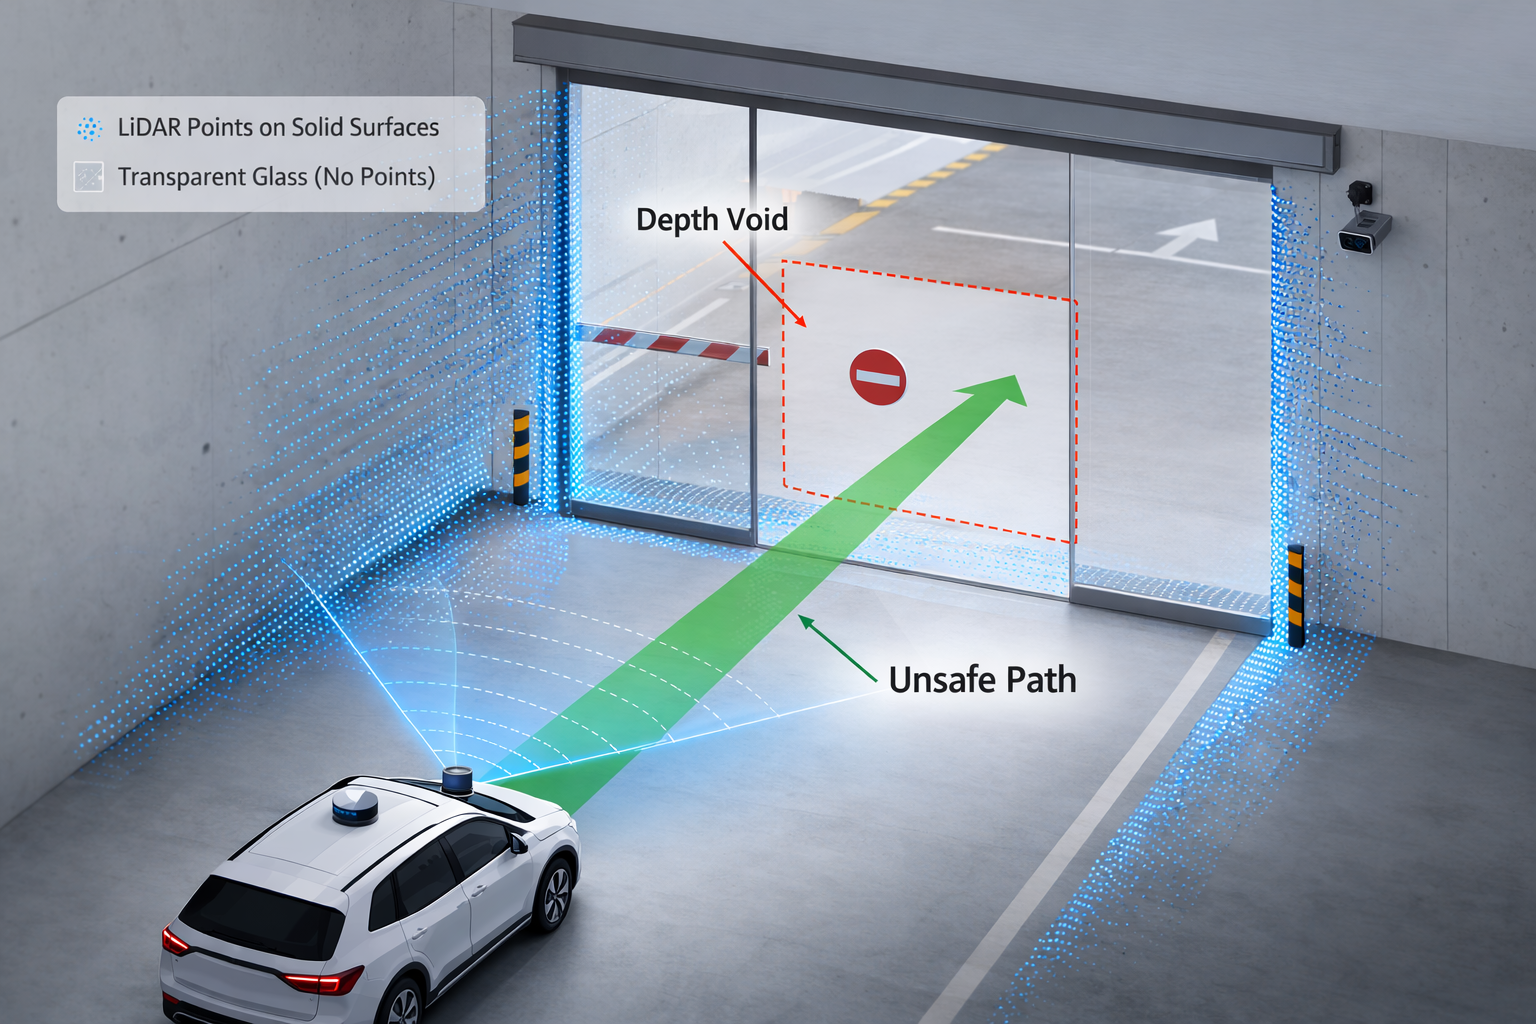
\includegraphics[width=\columnwidth]{A2_part_a_locked.png}
  \caption{A2 Transparent Garage Door (false-negative free-space) scenario. Visual background continuity is preserved through the closed glass door, while LiDAR depth certainty degrades at the true physical boundary. Unsafe behavior occurs when evidential uncertainty is aggressively collapsed into deterministic free-space.}
  \Description{A top-view and perspective illustration of A2 at a garage exit. The camera sees the outside street through a closed transparent glass door, while LiDAR fails to provide stable boundary depth, leading to false free-space inference.}
  \label{fig:a2}
\end{figure}

For each occupancy grid cell $c$, define an evidential frame $\Omega=\{O,F\}$ and mass function:
\begin{equation}
m_c(O)+m_c(F)+m_c(\Omega)=1,
\label{eq:a2_mass}
\end{equation}
where $m_c(\Omega)$ denotes unknown. A2 is triggered when uncertainty is prematurely collapsed into free-space:
\begin{equation}
m_c^{t+1}(F)=m_c^t(F)+\kappa m_c^t(\Omega),\quad
m_c^{t+1}(\Omega)=(1-\kappa)m_c^t(\Omega),
\label{eq:a2_collapse}
\end{equation}
with large $\kappa$ despite missing geometric confirmation.

\subsection{Part B: Placeholder for B1/B2 (To Be Filled by Teammate)}

\textbf{Reserved for teammate integration.} Keep the same structure as Part A:
\begin{itemize}
  \item B1 scenario definition, failure chain, architecture comparison, and risk.
  \item B2 scenario definition, transition-window failure chain, architecture comparison, and risk.
\end{itemize}

\section{Simulation \& Evaluation Setup}

\subsection{Part A: Phenomenological Simulation, Metrics, and Experimental Findings}

Part A uses a lightweight CPU-only 2D simulator (\texttt{NumPy}/\texttt{SciPy}) to isolate decision logic under contradictory evidence rather than photorealistic rendering. For each seed, both A1 and A2 are instantiated with domain randomization over geometry and sensing conditions (door position, transparency, depth-void span, initial speed, slope, and noise scale), then evaluated under three architectures: \textit{camera-only}, \textit{multimodal permissive}, and \textit{mitigation}. The evidential-map abstraction follows occupancy-grid and unknown-preserving mapping principles \cite{elfes2013,ufomap2020}.

For A1, we inject a persistent camera-dominant ghost hypothesis with weak or ambiguous auxiliary support. Safety severity is measured by Phantom Braking Severity (PBS):
\begin{equation}
\begin{aligned}
PBS &= \max_{t \in [t_0, t_{\text{end}}]}
\Big(\left|a_{\text{long}}(t)\right| \\
&\quad\cdot\mathbb{I}\big(TTC_{\text{virtual}}(t) < \tau_{\text{safe}} \land \text{No Physical Target}\big)\Big).
\end{aligned}
\label{eq:pbs}
\end{equation}
Across 100 randomized seeds, A1 PBS is $1.605$ (\textit{camera-only}), $1.933$ (\textit{multimodal permissive}), and $1.188$ (\textit{mitigation}), i.e., a $38.5\%$ reduction from permissive multi-modal to mitigation.

For A2, we use a Dempster-Shafer evidential grid and inject transparent-boundary depth voids while preserving strong visual free-space continuity. Evidential collapse is measured by EVR:
\begin{equation}
EVR =
\frac{1}{\left|\mathcal{G}_{\text{door}}\right|}
\sum_{c \in \mathcal{G}_{\text{door}}}
m_c^{t_{\text{cross}}}(F).
\label{eq:evr}
\end{equation}
The A2 results are intentionally extreme and informative: collision rate is $1.000$ for both \textit{camera-only} and \textit{multimodal permissive}, and $0.000$ for \textit{mitigation}; EVR decreases from $0.942$ (permissive multi-modal) to $0.104$ (mitigation). This should be interpreted as a system-level architecture finding: without explicit contradiction handling, semantic priors without robust geometric verification inevitably commit to false free-space under transparent barriers.

The three-stack comparison is also consistent with representative fusion families in the literature, including radar-camera fusion, transformer-based end-to-end fusion, and unified BEV fusion \cite{centerfusion2020,transfuser2021,bevfusion2022}. We additionally align the uncertainty-aware perspective with recent uncertainty-encoded fusion work \cite{umoe2023}. While this section does not train on large corpora, scenario parameters and modality assumptions are compatible with modern multi-sensor benchmarks such as nuScenes and Argoverse 2 \cite{caesar2020nuscenes,wilson2023argoverse2}.

Statistical significance is strong despite the deterministic-looking means. For A1 PBS (multimodal permissive vs mitigation), Mann-Whitney yields $p=1.08\times 10^{-13}$; for A2 EVR, $p=2.56\times 10^{-34}$; and for A2 collision rate, $p=3.52\times 10^{-45}$. Thus, the trends are not sampling artifacts of the 100-seed randomized protocol.

\begin{figure}[t]
  \centering
  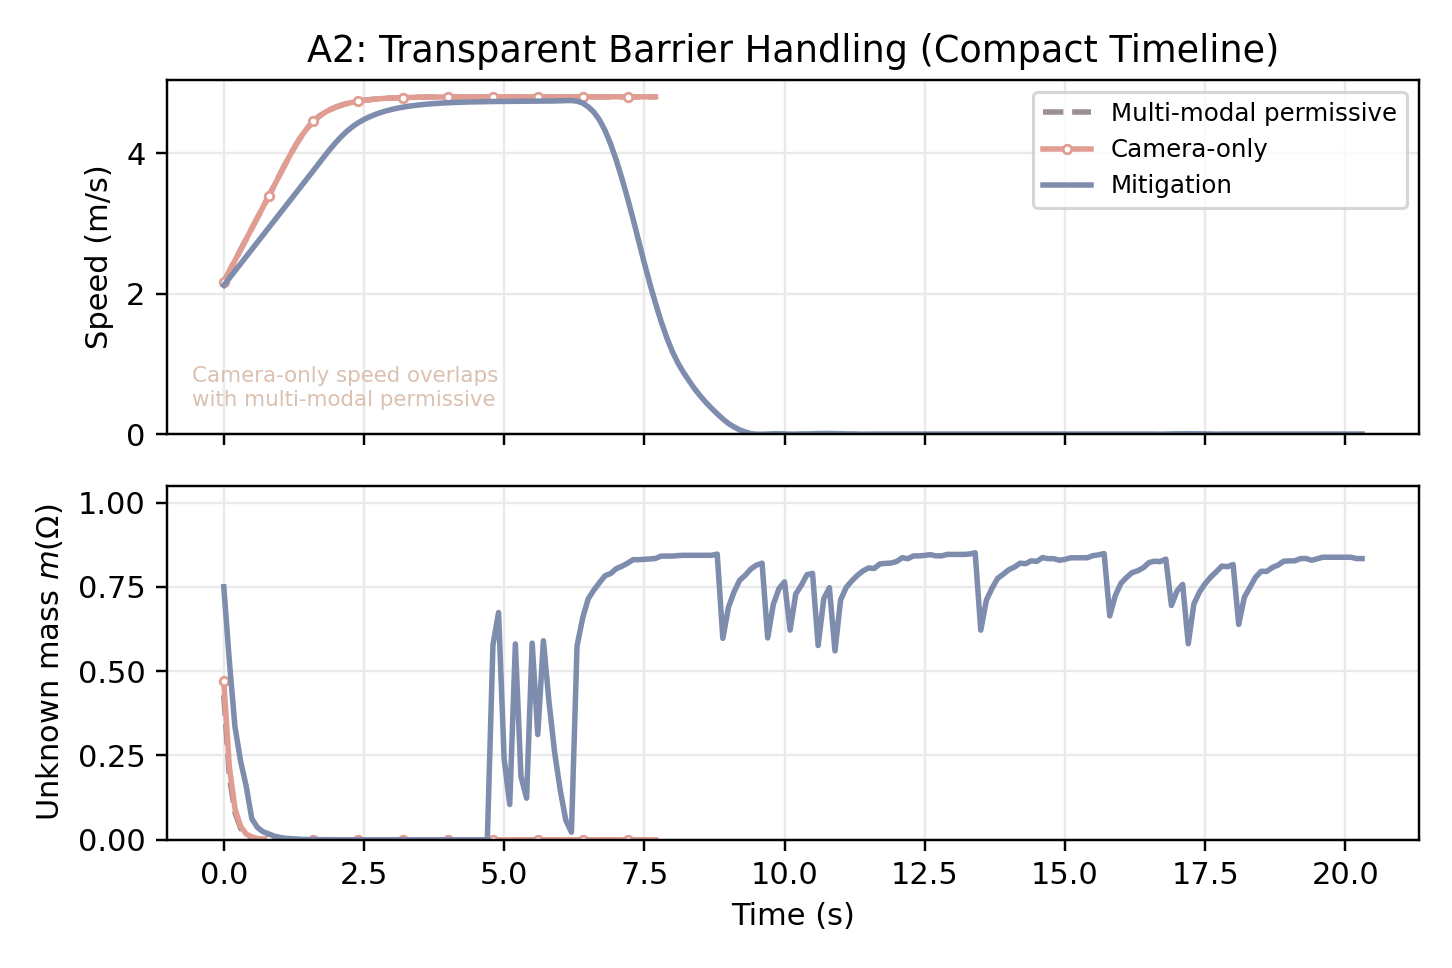
\includegraphics[width=\columnwidth]{../../results/part_a_simulation_100/a2_three_modes_timeline.png}
  \caption{A2 compact timeline (single-column). Top: speed profile; bottom: unknown evidential mass $m(\Omega)$ near the transparent boundary. Permissive baselines keep nominal motion under unresolved uncertainty and collide, whereas mitigation preserves uncertainty and enforces envelope-triggered deceleration to full stop.}
  \Description{Two-panel time-series plot for A2 under camera-only, multimodal permissive, and mitigation. The top panel shows speed over time; the bottom panel shows unknown evidential mass m(Omega). Baselines continue moving and collide; mitigation slows and stops under high uncertainty.}
  \label{fig:a2_timeline}
\end{figure}

\begin{table}[t]
  \caption{Part A cross-architecture results over 100 randomized seeds.}
  \label{tab:parta_pareto}
  \centering
  \small
  \setlength{\tabcolsep}{2.6pt}
  \renewcommand{\arraystretch}{1.10}
  \begin{tabular}{lcccc}
    \toprule
    Architecture & A1 PBS $\downarrow$ & A2 EVR $\downarrow$ & A2 Coll. $\downarrow$ & A2 $T_{\text{travel}}$ (s) $\uparrow$ \\
    \midrule
    Camera-only & 1.605 & 0.942 & 1.000 & 6.094 \\
    Multi-modal perm. & 1.933 & 0.942 & 1.000 & 6.094 \\
    Mitigation (ours) & 1.188 & 0.104 & 0.000 & 19.626 \\
    \bottomrule
  \end{tabular}
\end{table}

\subsection{Part B: Placeholder for Evaluation Setup}

\textbf{Reserved for teammate integration.} Include B1/B2 setup, metrics, and baseline-vs-mitigation matrix aligned with Part A reporting format.

\section{Mitigation Strategies}

\subsection{Part A: Mitigation Summary and Philosophy}

The core mitigation theme is a transition from \textit{semantic trust} to \textit{epistemic uncertainty management}. Section 4 shows that permissive architectures fail when contradictory evidence is forced into deterministic states. The proposed framework therefore intervenes at the fusion-to-planning interface \cite{huang2022survey}, treating unresolved cross-modal contradiction as a primary trigger for safety-critical fallback rather than as nuisance noise.

\subsubsection{A1 Mitigation: Variance-Penalized Fusion and Temporal Parallax}

To mitigate false-positive trajectory commitment near reflective facades (A1), the stack must break camera semantic dominance.

\textbf{Theoretical Prototype (2D Simulation):} We replace additive fusion with contradiction-aware evidential fusion (Eq.~\ref{eq:a1_penalized}), where cross-modal variance is explicitly penalized. In the 100-seed study, this reduces A1 PBS by $38.5\%$ versus the multi-modal permissive baseline.

\textbf{Multi-dimensional Real-World Extension:} In 3D deployment, spatial variance alone is insufficient because radar multipath can mimic geometric corroboration \cite{zheng2024radar}. A robust A1 mitigation should be extended along temporal and physical dimensions:
\begin{itemize}
  \item \textit{Temporal parallax consistency.} Real objects maintain motion and parallax consistency under ego motion, while reflections show anomalous kinematics (e.g., lateral slip or non-physical relative speed).
  \item \textit{Intensity/context profiling.} LiDAR intensity and local surface context can flag reflective facades \cite{zhao2024ref}, providing a contextual veto against persistent but unsupported visual tracks.
  \item \textit{Reflection-suppressed appearance priors.} Polarization-based reflection removal can reduce semantic contamination before detection and tracking \cite{polarfree2025}.
\end{itemize}

\subsubsection{A2 Mitigation: Evidential Preservation + Kinematic Envelope}

For transparent barriers (A2), mitigation preserves unknown evidential mass $m_c(\Omega)$ under depth dropouts and explicitly forbids premature collapse into free-space $m_c(F)$.

\textbf{Theoretical Prototype (2D Simulation):} To avoid deadlock under preserved uncertainty, we integrate an RSS-inspired kinematic envelope \cite{shalev2017}. The policy applies hysteresis creeping bounded by stopping distance:
\begin{equation}
a_{\text{eff}}=\max\!\left(0.8,\;a_{\text{max}}+g\sin\!\left(\theta_{\text{slope}}\right)\right),
\label{eq:a_eff}
\end{equation}
\begin{equation}
d_{\text{stop}}=\frac{v^2}{2a_{\text{eff}}}.
\label{eq:d_stop_mitigation}
\end{equation}

Algorithm~\ref{alg:rss_envelope} summarizes the online controller.
\begin{algorithm}[t]
\caption{Kinematic Safety Envelope under Evidential Uncertainty}
\label{alg:rss_envelope}
\begin{algorithmic}[1]
\Require Current velocity $v$, distance to boundary $d$, local unknown mass $m(\Omega)$, slope $\theta_{\text{slope}}$
\Ensure Target velocity $v_{\text{target}}$
\State $a_{\text{eff}} \gets \max(0.8,\; a_{\text{max}} + 9.81 \cdot \sin(\theta_{\text{slope}}))$
\State $d_{\text{stop}} \gets \dfrac{v^2}{2a_{\text{eff}}}$
\If{$m(\Omega) > \tau_{\text{uncertainty}}$}
  \If{$d \le d_{\text{stop}} + d_{\text{margin}}$}
    \State $v_{\text{target}} \gets 0$ \Comment{trigger maximum deceleration}
  \Else
    \State $v_{\text{target}} \gets v_{\text{creep}}$ \Comment{hysteresis creeping for disambiguation}
  \EndIf
\Else
  \State $v_{\text{target}} \gets v_{\text{nominal}}$
\EndIf
\State \Return $v_{\text{target}}$
\end{algorithmic}
\end{algorithm}

Within the 2D kinematic boundary model, this coupling of epistemic uncertainty and hard braking constraints reduces A2 collision rate from $1.000$ to $0.000$ over 100 randomized seeds.

\textbf{Multi-dimensional Real-World Extension:} The deterministic 2D result does not remove real-world nonlinearities:
\begin{itemize}
  \item \textit{Negative evidence modeling.} If scene priors imply a solid structure but LiDAR rays pass through without near returns, the \textit{absence} of expected returns should be encoded as positive transparent-barrier evidence rather than neutral missing data \cite{tibebu2021glass}. Learning-based geometry completion for transparent media also supports this design direction \cite{sajjanar2019cleargrasp}.
  \item \textit{Actuation latency.} Real braking introduces delay ($\tau_{\text{delay}}\approx 0.2\text{--}0.4\,\mathrm{s}$), so deployment envelopes should use
  \begin{equation}
  d_{\text{stop}}^{\text{real}} = v\,\tau_{\text{delay}} + \frac{v^2}{2a_{\text{eff}}}.
  \label{eq:d_stop_real}
  \end{equation}
\end{itemize}

\subsection{Part B: Placeholder for Mitigation Strategies}

\textbf{Reserved for teammate integration.} Include B1 lane-attribution robustness and B2 transition-state arbitration with hysteresis and dwell-time constraints.

\section{Challenges and Future Work}

The 0\% collision result for A2 mitigation is a bounded guarantee, not a claim of universal safety. It is valid within this simulator because actuation is modeled as near-instantaneous and longitudinal friction is represented by a bounded effective deceleration term. Real deployments include brake latency, tire-road friction variation, and slip effects that can violate the assumed stopping envelope.

A second challenge is conservatism. Preserving $m_c(\Omega)$ and enforcing envelope-triggered braking strongly improves safety, but materially reduces throughput in access zones. This is visible in the increased travel time and stop-time ratio under mitigation. Future work should therefore target adaptive conservatism: uncertainty-aware speed planning with context-dependent risk budgets, plus explicit comfort constraints on jerk.

Finally, future validation should expand beyond 2D kinematics toward higher-fidelity effects: asynchronous sensor timing, actuator lag models, variable friction, opening/closing door dynamics, and mixed static-dynamic interactions (e.g., pedestrians near transparent barriers). These additions are necessary to convert the current deterministic lower-bound argument into a more realistic probabilistic safety claim.

\section{Conclusion}

Across A1--B2, the dominant hazard is premature commitment under unresolved contradiction. The architecture-level comparison should therefore be evaluated as permissive commitment versus contradiction-aware commitment, rather than sensor-count comparison alone. Final conclusions and limitations for Part B will be merged after teammate integration.

\begin{thebibliography}{28}

\bibitem{nhtsa2024}
National Highway Traffic Safety Administration.
\newblock 2024.
\newblock \textit{Federal Motor Vehicle Safety Standards; Automatic Emergency Braking Systems for Light Vehicles (FMVSS No. 127)}.

\bibitem{euroncap2025}
Euro NCAP.
\newblock 2025.
\newblock \textit{Test Protocol: Crash Avoidance, Frontal Collisions, Version 11}.

\bibitem{huang2022survey}
K. Huang, C. Fu, and X. Wang.
\newblock 2022.
\newblock Multi-modal Sensor Fusion for Auto Driving Perception: A Survey.
\newblock \textit{arXiv preprint arXiv:2202.02703}.

\bibitem{zhao2024ref}
X. Zhao and S. Schwertfeger.
\newblock 2024.
\newblock 3DRef: 3D Dataset and Benchmark for Reflection Detection in RGB and Lidar Data.
\newblock \textit{arXiv preprint arXiv:2403.06538}.

\bibitem{li2024plane}
Y. Li, X. Zhao, and S. Schwertfeger.
\newblock 2024.
\newblock Detection and Utilization of Reflections in LiDAR Scans Through Plane Optimization and Plane SLAM.
\newblock \textit{arXiv preprint arXiv:2406.10494}.

\bibitem{tibebu2021glass}
H. Tibebu et al.
\newblock 2021.
\newblock LiDAR-Based Glass Detection for Improved Occupancy Grid Mapping and Object Detection.
\newblock \textit{Sensors} 21, 7 (2021), 2263.

\bibitem{weerakoon2024topgn}
K. Weerakoon et al.
\newblock 2024.
\newblock TOPGN: Real-time Transparent Obstacle Detection Using Lidar Point Cloud Intensity.
\newblock \textit{arXiv preprint arXiv:2408.05608}.

\bibitem{zheng2024radar}
L. Zheng et al.
\newblock 2024.
\newblock Detection of Ghost Targets for Automotive Radar in the Presence of Multipath.
\newblock \textit{IEEE Transactions on Signal Processing} 72 (2024), 2364--2379.

\bibitem{mutcd2023}
Federal Highway Administration.
\newblock 2023.
\newblock \textit{Manual on Uniform Traffic Control Devices (MUTCD), 11th Edition}.

\bibitem{fhwa2019}
Federal Highway Administration.
\newblock 2019.
\newblock \textit{Traffic Simulation Assessment of New and Reconstructed Two-Way Left-Turn Lane Reversal Configurations}, FHWA-HRT-19-025.

\bibitem{fhwa2008}
Federal Highway Administration.
\newblock 2008.
\newblock \textit{Signalized Intersections: Informational Guide}, FHWA-HRT-04-091.

\bibitem{manuel2020}
A. Manuel, A. de Barros, and R. Tay.
\newblock 2020.
\newblock Traffic safety meta-analysis of reversible lanes.
\newblock \textit{Accident Analysis \& Prevention} 148 (2020), 105751.

\bibitem{behrendt2017}
K. Behrendt and L. Novak.
\newblock 2017.
\newblock A deep learning approach to traffic lights: Detection, tracking, and classification.
\newblock In \textit{Proc. IEEE ICRA}.

\bibitem{jensen2018}
M. Jensen et al.
\newblock 2018.
\newblock The DriveU Traffic Light Dataset: Introduction and Comparison with Existing Datasets.
\newblock In \textit{Proc. IEEE ICRA}.

\bibitem{hirabayashi2019}
M. Hirabayashi et al.
\newblock 2019.
\newblock Traffic light recognition using high-definition map features.
\newblock \textit{Robotics and Autonomous Systems} 111 (2019), 62--72.

\bibitem{monninger2023}
M. Monninger et al.
\newblock 2023.
\newblock Traffic-Light-to-Lane Assignment in Structured Urban Environments.
\newblock \textit{arXiv preprint arXiv:2309.12087}.

\bibitem{veer2022}
S. Veer et al.
\newblock 2022.
\newblock Receding Horizon Planning with Rule Hierarchies for Autonomous Vehicles.
\newblock \textit{arXiv preprint arXiv:2212.03323}.

\bibitem{shalev2017}
S. Shalev-Shwartz, S. Shammah, and A. Shashua.
\newblock 2017.
\newblock On a Formal Model of Safe and Scalable Self-driving Cars.
\newblock \textit{arXiv preprint arXiv:1708.06374}.

\bibitem{elfes2013}
A. Elfes.
\newblock 2013.
\newblock Occupancy Grids: A Stochastic Spatial Representation for Active Robot Perception.
\newblock \textit{arXiv preprint arXiv:1304.1098}.

\bibitem{ufomap2020}
D. Duberg and P. Jensfelt.
\newblock 2020.
\newblock UFOMap: An Efficient Probabilistic 3D Mapping Framework That Embraces the Unknown.
\newblock \textit{arXiv preprint arXiv:2003.04749}.

\bibitem{centerfusion2020}
R. Nabati and H. Qi.
\newblock 2020.
\newblock CenterFusion: Center-based Radar and Camera Fusion for 3D Object Detection.
\newblock \textit{arXiv preprint arXiv:2011.04841}.

\bibitem{transfuser2021}
A. Prakash, K. Chitta, and A. Geiger.
\newblock 2021.
\newblock Multi-Modal Fusion Transformer for End-to-End Autonomous Driving.
\newblock \textit{arXiv preprint arXiv:2104.09224}.

\bibitem{bevfusion2022}
Z. Liu et al.
\newblock 2022.
\newblock BEVFusion: Multi-Task Multi-Sensor Fusion with Unified Bird's-Eye View Representation.
\newblock \textit{arXiv preprint arXiv:2205.13542}.

\bibitem{umoe2023}
Y. Lou, Q. Song, Q. Xu, R. Tan, and J. Wang.
\newblock 2023.
\newblock Uncertainty-Encoded Multi-Modal Fusion for Robust Object Detection in Autonomous Driving.
\newblock \textit{arXiv preprint arXiv:2307.16121}.

\bibitem{caesar2020nuscenes}
H. Caesar et al.
\newblock 2020.
\newblock nuScenes: A Multimodal Dataset for Autonomous Driving.
\newblock In \textit{Proc. IEEE/CVF CVPR}.

\bibitem{wilson2023argoverse2}
B. Wilson et al.
\newblock 2023.
\newblock Argoverse 2: Next Generation Datasets for Self-Driving Perception and Forecasting.
\newblock \textit{arXiv preprint arXiv:2301.00493}.

\bibitem{polarfree2025}
M. Yao, M. Wang, K.-M. Tam, L. Li, T. Xue, and J. Gu.
\newblock 2025.
\newblock PolarFree: Polarization-based Reflection-Free Imaging.
\newblock In \textit{Proc. IEEE/CVF CVPR}.

\bibitem{sajjanar2019cleargrasp}
S. S. Sajjanar et al.
\newblock 2019.
\newblock ClearGrasp: 3D Shape Estimation of Transparent Objects for Manipulation.
\newblock \textit{arXiv preprint arXiv:1910.02550}.

\end{thebibliography}

\end{document}
